\documentclass[UTF8,a4paper]{article}
\usepackage{ctex}
\usepackage{graphicx}
\graphicspath{{image/}}
\title{梯度下降}
\author{Luke}
\begin{document}
\maketitle

梯度下降算法中,步长(学习率,$\eta$)的选取是很重要的一个问题。步长太小会导致 Loss function 下降得很慢,步长太大又会导致 Loss function 不能到达最低点甚至越走越大。解决这个问题的方法是采用自适应的步长(Adaptive Learing Rate):初始点一般距离目标比较远,此时可以用比较大的步长,当距离目标比较近的时候,选用比较小的步长。

\section{Adagrad}

Adagrad 是比较容易实现的一种方法。将每个参数的步长除以之前的所有的微分值的平方均根:

\paragraph{普通的梯度下降}
\begin{equation}
w^{t+1}\leftarrow w^{t}-\eta^t g^t
\end{equation}

\paragraph{Adagrad}
\begin{equation}
w^{t+1}\leftarrow w^t- \frac{\eta^t}{\sigma^t}g^t
\end{equation}

其中,$\eta^t=\frac{\eta}{\sqrt{t+1}},g^t=\frac{\partial L(w^t)}{\partial w^t}$

例如:
\[w^1\leftarrow w^0-\frac{\eta^0}{\sigma^0} g^0 \quad \sigma^0=\sqrt{(g^0)^2}\]

\[w^2\leftarrow w^1-\frac{\eta^1}{\sigma^1}g^1 \quad \sigma^1=\sqrt{\frac{1}{2}[(g^0)^2+(g^1)^2]}  \]

\begin{center}
$\dots\dots$
\end{center}

\[w^{t+1}\leftarrow w^t-\frac{\eta^t}{\sigma^t}g^t \quad \sigma^t=\sqrt{\frac{1}{t+1}\sum^t_{i=0}(g^i)^2}\]

\[w^{t+1}\leftarrow w^t-\frac{\frac{\eta}{\sqrt{t+1}}}{\sqrt{\frac{1}{t+1}\sum^t_{i=0}(g^i)^2}}g^t\]


\[\Downarrow\]
 

\begin{equation}
w^{t+1}\leftarrow w^t-\frac{\eta}{\sqrt{\sum^t_{i=0}(g^i)^2}}g^t
\end{equation}

\section{Stochastic Gradient Descent}

对于普通梯度下降:

\[L=\sum_n \left(\hat{y}^n-\left(b+\sum w_i x_i^n\right)\right)^2\qquad w^i=w^{i-1}-\eta\nabla L(w^{i-1})\]

Stochastic Gradient Descent: 选择一个$x^n$

\begin{equation}
L^n=\left(\hat{y}^n-\left(b+\sum w_i x_i^n\right)\right)^2 \qquad w^i=w^{i-1}-\eta\nabla L^n(w^{i-1})
\end{equation}

\begin{figure}[ht]
\centering
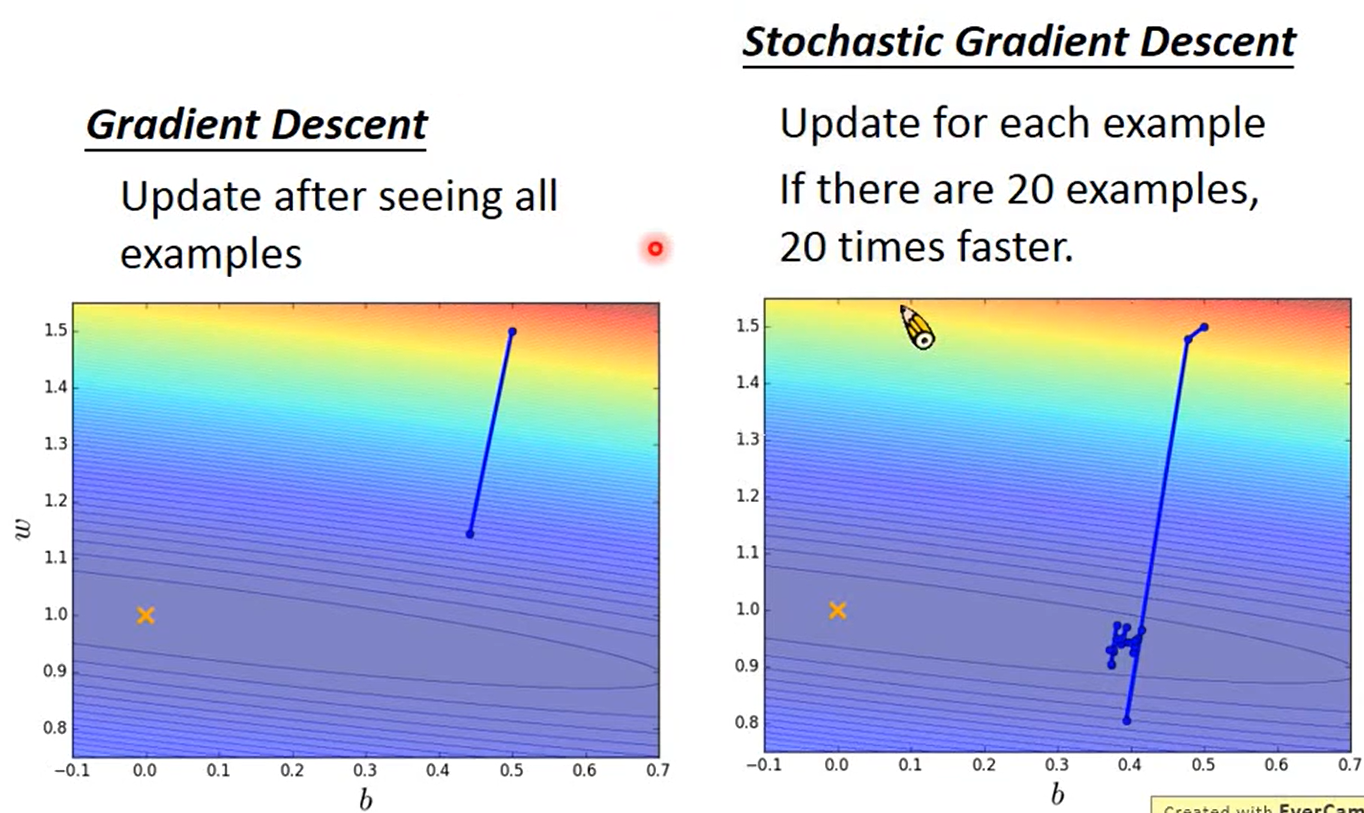
\includegraphics[width=300pt]{stochasticGradientDescent.png}
\caption{两种方法计算速度的对比}
\label{stochastic}
\end{figure}

\section{Feature Scaling (归一化)}

模型中有多个参数时,不同参数间的数值关系也会影响到梯度下降的计算速度。

\newpage

\begin{figure}[ht]
\centering
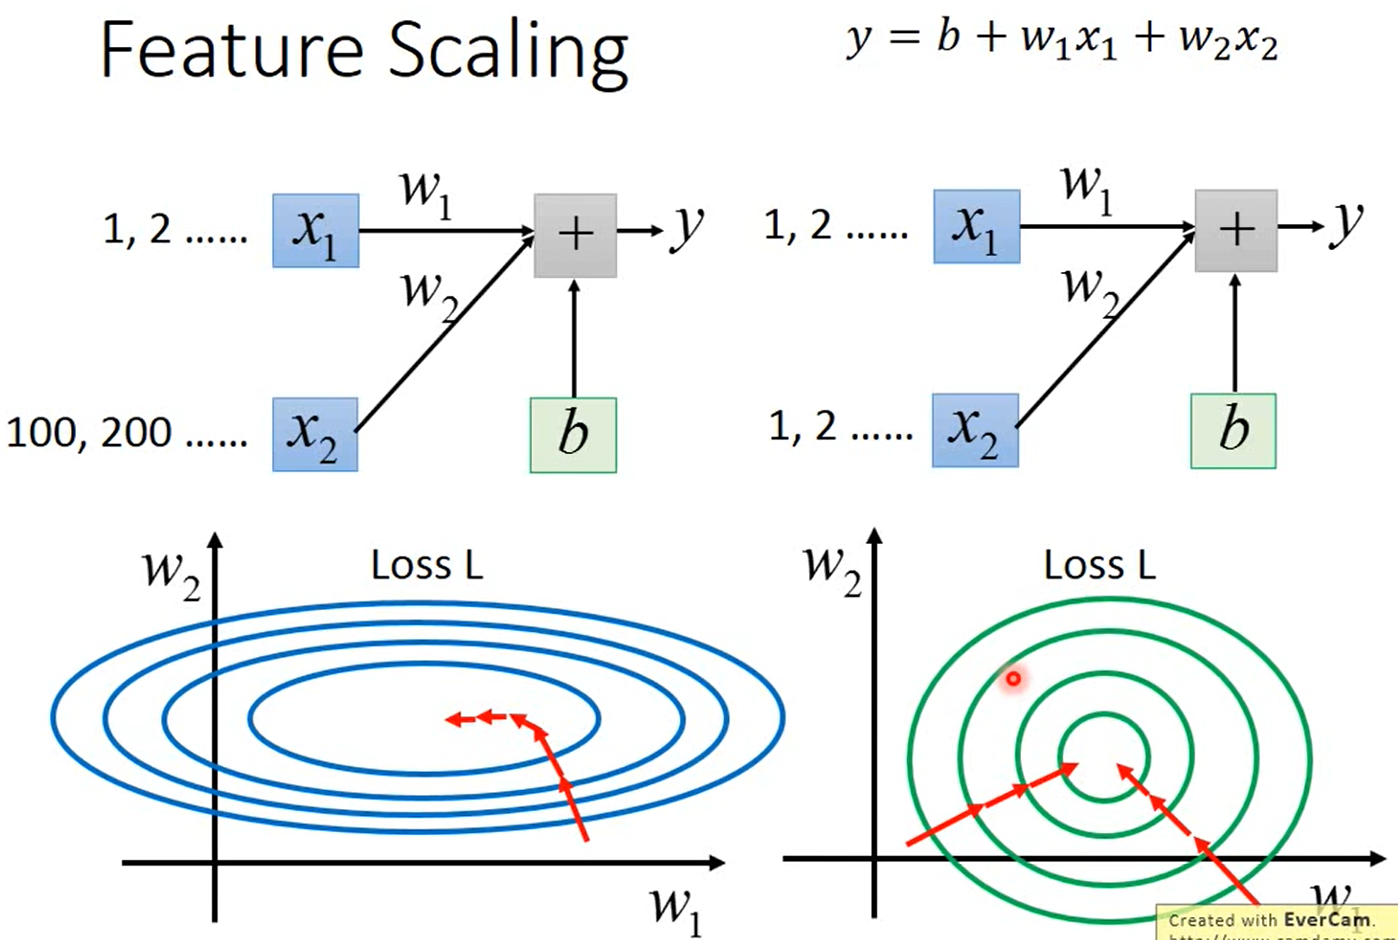
\includegraphics[width=340pt]{featureScaling.png}
\caption{参数的均值与方差对梯度下降算法的影响}
\label{featureScaling}
\end{figure}

常见的归一化方法是对每组数据的同一维度下的坐标进行计算,算出均值与方差,再基于此归一化(如图3):

\begin{figure}[ht]
\centering
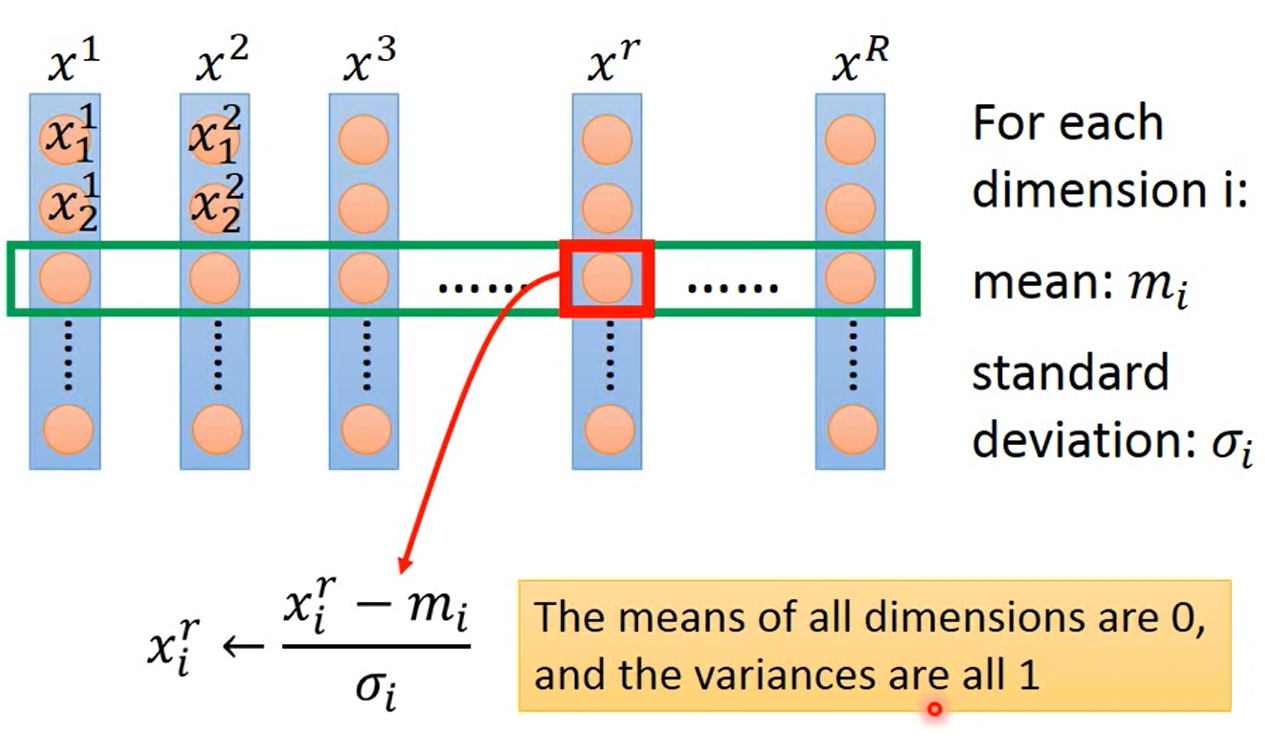
\includegraphics[width=260pt]{scalingMethod.png}
\caption{归一化方法}
\label{scalingMethod}
\end{figure}

\newpage

\section{局限性}

\begin{figure}[ht]
\centering
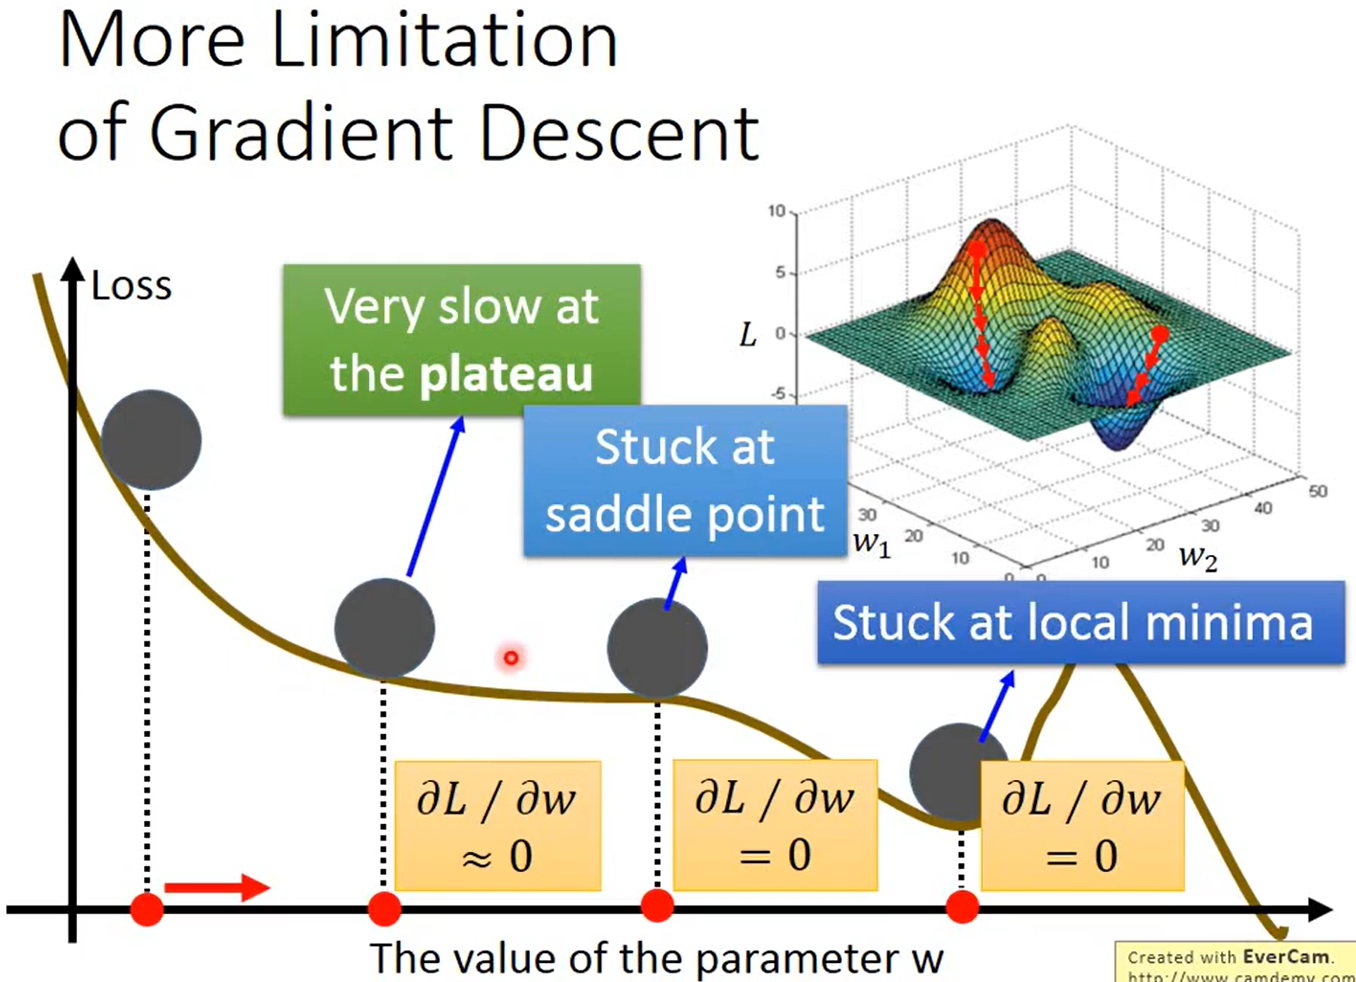
\includegraphics[width=340pt]{limitation.png}
\caption{梯度下降方法的局限性}
\label{limitation}
\end{figure}

梯度下降方法可能会被困在极点、马鞍点,导致找不到最小点。或者在斜率很小的地方,由于算力限制,Loss下降得非常缓慢,也容易被困住。

\end{document}